\section{Experimental Study}
\label{sec:exp}
In this section, we present the experimental setup in \cref{sec:exp:setup} and investigate the following research questions: 
% \ding{172} Compare the overall performance against baseline algorithms on full ranking (\cref{sec:exp:full}) and \LIMIT~$K$ (\cref{sec:exp:topk}); 
% \ding{173} Conduct an ablation study on \SLT (\cref{sec:exp:ablation});
% \ding{174} Validate the three cost models by varying the fan-in $k$ (\cref{sec:exp:cost});
% \ding{175} Investigate the impact of listwise batch size on performance (\cref{sec:exp:m}).
\textbf{RQ1.} How does our approach compare with baseline algorithms in ranking quality and efficiency for full ranking  (\cref{sec:exp:full}) and \LIMIT $K$ (\cref{sec:exp:topk})?
\textbf{RQ2.} How does the segmented loser tree save tokens and latency (\cref{sec:exp:ablation})?
\textbf{RQ3.} Do the proposed cost models accurately characterize the empirical token cost as the fan-in $k$ varies (\cref{sec:exp:cost})?
\textbf{RQ4.} How does the listwise batch size affect ranking performance and token cost (\cref{sec:exp:m})? 

\begin{table}[t]
\caption{Statistics of evaluation datasets.}
\label{tab:datasets}
\centering
\footnotesize
\setlength{\tabcolsep}{2.5pt}
\begin{tabular}{c l r l c}
\toprule
\textbf{Benchmark} & \textbf{Dataset} & $|D|$ & \textbf{Domain} & \textbf{\#~Queries} \\
\midrule
SemBench & \Movies & 86K & Movie information and reviews & 1\\ 
\midrule
\multirow{2}{*}{TREC} & \DLtwozero & 8.8M & Web passage retrieval & 54\\
& \DLtwotwo & 138M & Web passage retrieval (v2) & 25 \\
\midrule
\multirow{3}{*}{BEIR} & \COVID & 171K & Biomedical literature retrieval & 25\\
& \Touche & 382K & Argument retrieval & 25\\
& \FiQA & 57K & Financial QA retrieval & 25\\
\bottomrule
\end{tabular}
\end{table}

\subsection{Experimental Setup}
\label{sec:exp:setup}

\stitle{Datasets.}
Table~\ref{tab:datasets} summarizes the six datasets used in our experiments. 
% These datasets cover diverse semantic ranking scenarios, including general semantic search, web passage retrieval, and domain-specific information retrieval. 
\Movies is from SemBench~\cite{lao2026sembench}, a benchmark for evaluating semantic query processing systems. \DLtwotwo~\cite{arxiv21trecdl20} and \DLtwozero~\cite{arxiv25trecdl22} are large-scale passage retrieval benchmarks built on the MS MARCO corpus, widely used for evaluating query-passage ranking in web search and RAG systems. 
We further include three datasets from the BEIR ~\cite{arxiv21BEIR} benchmark, including \COVID for biomedical literature retrieval, \Touche for argument retrieval, and \FiQA for financial question answering retrieval. These datasets span multiple domains and scales, providing comprehensive evaluation across different semantic ranking scenarios.




\noindent\textbf{Baselines.}
We compare against 7 baseline algorithms. 
Here, Pointwise, External Pointwise, External Bubble, and External Merge are open-source LLM-based ranking algorithms~\cite{DBLP:journals/corr/abs-2509-00303}. 
LMPQSort, LMPQSelect, and Tournament are the listwise semantic \textsf{ORDER BY} algorithms in the ListK framework~\cite{DBLP:journals/corr/abs-2603-17223}. 
Quicksort is the algorithm in Lotus~\cite{DBLP:journals/pvldb/PatelJPGAGZ25}. 
Table~\ref{tab:ranking-algorithms} summarizes the type and asymptotic complexity\footnote{For Tournament, $b_m=(n-1)/(m-1)$ and $\ell_m=\log(n/m)$.
For LMPQSort/Select, $p$ is the pivot count,
$\kappa=K/n$, $\chi_p=(m-p)\log(p+1)$, and
$\psi_p(\kappa)=(m-p)[p-1+\kappa^{p+1}+(1-\kappa)^{p+1}]$. For our algorithms, $r = r_0 = \lceil n/m\rceil$.} regarding LLM calls for these 7 algorithms, together with our sliding window (\SD), loser tree (\LT) and segmented loser tree (\SLT) merge algorithms. 
%We compare these algorithms for both full ranking and \LIMIT~$K$. 


% Four-column candidate for Table 3.  Superscripts encode implementation
% provenance; keep formulas aligned with the five-column candidate.
\begin{table}[t]
\centering
\scriptsize
\caption{Summary of algorithms and their
complexity}
\label{tab:ranking-algorithms}
\setlength{\tabcolsep}{1.5pt}
%\renewcommand{\arraystretch}{1.12}
\begin{tabular}{l c c c }
% \begin{tabularx}{\columnwidth}{
%   @{}
%   >{\raggedright\arraybackslash}p{1.72cm}
%   >{\centering\arraybackslash}p{0.92cm}
%   >{\centering\arraybackslash}X
%   >{\centering\arraybackslash}X
%   @{}
% }
\toprule
\textbf{Algorithm} & \textbf{Type}
& \makecell[c]{\textbf{Full Rank} \textbf{Calls}}
& \makecell[c]{\textbf{\LIMIT $K$} \textbf{Calls}} \\
\midrule
Pointwise & Pointwise
& $\mathcal{O}(n)$
& $\mathcal{O}(n)$ \\
\makecell[l]{External Pointwise} & Pointwise
& $\mathcal{O}(n/m)$
& $\mathcal{O}(n/m)$ \\
\makecell[l]{External Bubble} & Listwise
& $\mathcal{O}(n^2/m^2)$
& $\mathcal{O}(Kn/m^2)$ \\
\makecell[l]{External Merge} & Listwise
& $\mathcal{O}((n/m)[1+ \ell_m])$
& $\mathcal{O}((n/m)[2+\log(K/m)])$ \\
\midrule
\makecell[l]{LMPQSort/Select} & Listwise
& $\mathcal{O}(n\log n/\chi_p+n)$
& $\mathcal{O}((p+1)n/\psi_p(\kappa))$ \\
Tournament & Listwise
& $\mathcal{O}\!\left(b_m+(n-1) \ell_m\right)$
& $\mathcal{O}\!\left(b_m+(K-1)\ell_m\right)$ \\
\midrule
Quicksort & Pairwise
& $\mathcal{O}(n\log n)$
& $\mathcal{O}\!\left(n+K\log K\right)$ \\
\midrule
\makecell[l]{Sliding Window} & Listwise
& $\mathcal{O}(r+nP(k)/\mu_{\SD}(k,m))$
& $\mathcal{O}(r+KP(k)/\mu_{\SD}(k,m))$ \\
Loser Tree  & Listwise
& $\mathcal{O}(r+nP(k))$
& $\mathcal{O}(r+KP(k))$ \\
Segmented Loser Tree & Listwise
& $\mathcal{O}(r+nP(k)/h)$
& $\mathcal{O}(r+KP(k)/h)$ \\
\bottomrule
\end{tabular}
% \vspace{1.5pt}

% \begin{minipage}{\columnwidth}
% \tiny\raggedright
% For Tournament, $b_m=(n-1)/(m-1)$ and $\ell_m=\log(n/m)$.
% For LMPQSort/Select, $p$ is the pivot count,
% $\kappa=K/n$, $\chi_p=(m-p)\log(p+1)$, and
% $\psi_p(\kappa)=(m-p)[p-1+\kappa^{p+1}+(1-\kappa)^{p+1}]$.
% % $r$, $h$, $P(k)$, and $\mu_k$ follow Table~\ref{tab:params-full}, with
% % $g=k$ for $\mu_k$.
% \end{minipage}
\end{table}






\noindent\textbf{Evaluation Metrics.}
% We evaluate the accuracy of these algorithms for both full ranking and \LIMIT~$K$.
For full ranking, we use Spearman's rank correlation coefficient $\rho$ between the predicted order and the ground-truth order.
For \LIMIT~$K$, we adopt the normalized Discounted Cumulative Gain (nDCG@$K$), which is a widely used information retrieval metric for top-$K$ ranking. 
Each algorithmic configuration is tested by 10 independent runs on all the queries in one benchmark in Table~\ref{tab:datasets}, and the overall average results are reported.

\noindent\textbf{Implementation Details.}
All the algorithms are empowered by vLLM~\cite{kwon2023efficient} that invokes Qwen3-32B~\cite{DBLP:journals/corr/abs-2505-09388} with a tensor parallelism degree of 8 (tensor\_parallel\_size=8). All experiments are conducted on a Linux server equipped with dual AMD EPYC 9554 CPUs (64 cores, 512 GB RAM) and 8 NVIDIA RTX 5090 GPUs.
Our algorithms are implemented in Python and Pandas. 
By default, we use the cost models in \cref{sec:cost} to select fan-in $k$ for full ranking, and an empirical $k$ for \LIMIT $K$.
The prompt for listwise calls in different algorithms is aligned with the prompt of the baseline algorithm~\cite{DBLP:journals/corr/abs-2509-00303}.

\subsection{Overall Performance of Full Ranking}
\label{sec:exp:full}

\begin{table*}[t]
\centering\footnotesize
\caption{Comparison of Spearman coefficient ($\rho$) or nDCG@10, \#Tok. ($\times 10^3$), and Lat. (seconds) on full ranking. (The best and second-best values are in \textbf{bold} and \underline{underlined}, respectively. Avg. Rank denotes the algorithms' average rank across datasets)}
\label{tab:exp1-full}
\setlength{\tabcolsep}{2pt}
\begin{tabular}{@{}lrrrrrrrrrrrrrrrrrrrrr@{}}
\toprule
 & \multicolumn{3}{c}{\Movies} & \multicolumn{3}{c}{\DLtwozero} & \multicolumn{3}{c}{\DLtwotwo} & \multicolumn{3}{c}{\COVID} & \multicolumn{3}{c}{\Touche} & \multicolumn{3}{c}{\FiQA} & \multicolumn{3}{c}{Avg. Rank} \\
\cmidrule(lr){2-4} \cmidrule(lr){5-7} \cmidrule(lr){8-10} \cmidrule(lr){11-13} \cmidrule(lr){14-16} \cmidrule(lr){17-19} \cmidrule(lr){20-22}
Algorithm & $\rho$ & \#Tok. & Lat. & $\rho$ & \#Tok. & Lat. & $\rho$ & \#Tok. & Lat. & $\rho$ & \#Tok. & Lat. & $\rho$ & \#Tok. & Lat. & nDCG & \#Tok. & Lat. & $\rho$/nDCG & \#Tok. & Lat. \\
\midrule
Pointwise & 0.733 & \underline{26.6} & \underline{2.2} & 0.419 & \underline{25.2} & \underline{3.5} & 0.374 & \underline{23.4} & \underline{2.4} & 0.392 & \underline{44.8} & \underline{5.3} & 0.479 & \underline{69.0} & \underline{9.3} & 0.373 & \underline{44.9} & \underline{5.6} & 10 & \underline{2} & \underline{2} \\
Ext. Pointwise & 0.770 & \textbf{13.0} & \textbf{0.8} & 0.457 & \textbf{14.3} & \textbf{2.6} & 0.363 & \textbf{12.4} & \textbf{1.7} & 0.449 & \textbf{33.4} & \textbf{4.6} & 0.381 & \textbf{57.9} & \textbf{8.9} & 0.378 & \textbf{33.3} & \textbf{4.8} & 9 & \textbf{1} & \textbf{1} \\
Ext. Bubble & \underline{0.782} & 296.8 & 147.2 & \textbf{0.572} & 278.6 & 142.8 & 0.461 & 238.4 & 103.4 & 0.396 & 504.2 & 137.9 & \textbf{0.537} & 1100.3 & 232.9 & 0.461 & 656.9 & 175.3 & \underline{2} & 10 & 10 \\
Ext. Merge & 0.777 & 69.8 & 18.8 & 0.528 & 72.7 & 24.3 & 0.423 & 61.3 & 19.2 & 0.480 & 177.0 & 40.1 & 0.410 & 294.8 & 142.8 & 0.455 & 171.9 & 36.0 & 7 & 6 & 6 \\
\midrule
LMPQSort & \textbf{0.787} & 78.3 & 19.7 & 0.534 & 80.0 & 23.9 & 0.377 & 60.5 & 15.7 & \textbf{0.522} & 191.0 & 47.9 & 0.438 & 311.1 & 112.8 & 0.447 & 188.2 & 35.8 & 6 & 8 & 5 \\
Tournament & 0.763 & 72.0 & 26.8 & 0.522 & 68.0 & 27.7 & 0.408 & 61.2 & 21.9 & \underline{0.500} & 134.6 & 51.9 & 0.395 & 202.5 & 40.5 & 0.450 & 131.3 & 32.8 & 8 & 5 & 7 \\
\midrule
Quicksort & 0.741 & 297.4 & 19.3 & \underline{0.559} & 244.5 & 21.1 & \textbf{0.480} & 234.4 & 19.1 & 0.454 & 462.3 & 60.5 & 0.442 & 731.8 & 129.5 & 0.453 & 479.1 & 38.3 & 5 & 9 & 8 \\
\midrule
Sliding Window & 0.760 & 63.5 & 18.9 & 0.552 & 67.5 & 18.5 & \underline{0.470} & 57.0 & 16.8 & 0.492 & 148.7 & 29.2 & \underline{0.518} & 248.4 & 43.2 & 0.493 & 143.8 & 26.9 & \textbf{1} & 4 & 3 \\
Loser Tree & 0.771 & 86.7 & 32.6 & 0.544 & 82.9 & 28.5 & 0.462 & 73.6 & 26.4 & 0.462 & 160.0 & 39.4 & 0.411 & 266.6 & 54.3 & \textbf{0.503} & 170.6 & 39.0 & 3 & 7 & 9 \\
Segmented Loser Tree & 0.771 & 63.9 & 25.3 & 0.542 & 64.8 & 22.1 & 0.452 & 56.9 & 22.1 & 0.452 & 140.5 & 33.6 & 0.445 & 246.9 & 47.6 & \underline{0.497} & 145.7 & 32.4 & 4 & 3 & 4 \\
\bottomrule
\end{tabular}
\end{table*}

\Cref{tab:exp1-full} reports the full ranking performance of our three merge algorithms, \SD, \LT, and \SLT, together with seven baselines under the default configurations specified in \cref{sec:exp:setup}. We evaluate token count, ranking quality, and latency on all six datasets and \textit{Avg. Rank} denotes the mean rank of an algorithm across the six datasets, providing a summary of its overall performance.
For \Movies, we evaluate Query~9 over 15 independent runs. 
For \DLtwozero, we evaluate all 54 queries with 10 runs per query; for each of the remaining four datasets, we evaluate a 25-query subset with 10 runs per query. 
For \FiQA, we report nDCG@10 instead of Spearman correlation, as its sparse relevance labels make top-ranked retrieval quality a more appropriate measure than global rank correlation.
All reported values are averaged over the evaluated queries and runs.

\noindent \textbf{Overall Comparison.}
Our methods achieve a strong trade-off among token count, ranking quality, and latency.
Compared with other listwise algorithms, our three algorithms incur the lowest token count while maintaining competitive latency and superior quality.
Pointwise baselines achieve lower token count and latency, but at a substantial compromise in ranking quality.
Ext. Bubble delivers comparable ranking quality but requires substantially greater computational cost. Overall, our methods obtain better average ranks than Ext. Merge, LMPQSort, and Tournament across the three evaluation dimensions.

\noindent \textbf{Quality--Cost Analysis.}
The performance differences arise primarily from how each method exploits the model context. 
Pointwise methods process items independently and therefore fail to capture the global relative information required for accurate ranking.
Although this design minimizes token consumption and latency, it results in the lowest ranking quality.
Ext. Bubble achieves strong quality but incurs high cost because its pairwise invocation pattern underutilizes the large context window and introduces redundant comparisons.
In contrast, our methods employ a $k$-way merge strategy with an automated cost model that selects the appropriate fan-in. 
This design better utilizes the listwise context, preserving high ranking quality while substantially reducing token consumption relative to merge-based baselines such as Ext. Merge and Tournament.
These results demonstrate the effectiveness of cost-aware merging for efficient listwise ranking.




% \stitle{Our algorithms sit on the quality--cost frontier.}
% \SD attains the best quality outright on \DLtwotwo, and \SLT on \FiQA. 
% On the remaining four datasets our best algorithms metains comparable quality of the best baseline while spending a fraction of its tokens.
% For average quality rank of \cref{tab:exp1-full}, \SD places first among all ten methods and \LT places third, with only LMPQSort in between.

% \stitle{Cheap scans give up substantial quality.} External Pointwise is always the cheapest method, but
% its quality trails the best method by 0.07--0.12 on the three.  
% Only on \LT, whose ordering criterion is well
% captured by independent scalar scores, does it come close. Lotus Quicksort combines high token cost with the lowest quality throughout, as its pivot comparisons
% repeatedly re-embed long documents.

% \stitle{Among our algorithmss.}
% \SD is the strongest on four datasets, \LT leads on
% \Movies, and \SLT on \FiQA. \LT stays within 0.013 of the best of our algorithmss on \Movies, \DLtwozero, and \DLtwotwo, but trails by 0.026--0.056 on the three BEIR collections.
% \SLT is cheaper \LT on every dataset, but pays in full-ranking
% quality on \Movies, \DLtwozero, and
% \COVID; \cref{sec:exp:ablation} isolates this
% trade-off, and \cref{sec:exp:m} shows it narrows at larger $m$.

% \stitle{Where baselines win.}
% We report the remaining losses plainly. On \Movies, LMPQSort attains the
% best quality (0.787 at 78.3K tokens vs.\ \LT's 0.771 at 86.7K); on
% \DLtwozero, External Bubble reaches 0.572 against 0.557 of \SD at
% $4.2\times$ the token cost; and on \COVID and \Touche, LMPQSort and Pointwise edge out \SD.
% On the remaining two datasets, one of our algorithmss attains the highest
% reported quality.

% \stitle{Latency is the price of sequential emission.}
% Our three merge algorithms are roughly an order of magnitude slower per sort. The cause is structural: within a merge group each listwise
% call depends on the previous emission, and the final pass is a single group,
% so calls serialize; baselines instead batch many independent calls.
% Token cost---the billed resource and the objective of
% \cref{sec:cost}---is unaffected, groups within early passes still run in
% parallel, and \LIMIT~$K$ removes most of the gap
% (\cref{sec:exp:topk}). Making the final pass latency-competitive (e.g., by
% overlapping refresh calls) is left as future work.

\subsection{Overall Performance under \LIMIT~$K$}
\label{sec:exp:topk}

\newcommand{\pendingviz}[1]{%
  \par\medskip\noindent\fbox{\begin{minipage}{0.92\linewidth}\centering\small
  \textit{Pending approved layout: #1}\end{minipage}}\par\medskip
}

\begin{table*}[t]
\centering\footnotesize
\caption{Comparison of nDCG@10, \#Tok. ($\times 10^3$), and latency (seconds) on \LIMIT~$K$. (The best and second-best values are in \textbf{bold} and \underline{underlined}, respectively. Avg. Rank denotes the algorithm's average rank across datasets).}
\label{tab:exp1-topk}
\setlength{\tabcolsep}{2.5pt}
\begin{tabular}{@{}lrrrrrrrrrrrrrrrrrrrrr@{}}
\toprule
 & \multicolumn{3}{c}{\Movies} & \multicolumn{3}{c}{\DLtwozero} & \multicolumn{3}{c}{\DLtwotwo} & \multicolumn{3}{c}{\COVID} & \multicolumn{3}{c}{\Touche} & \multicolumn{3}{c}{\FiQA} & \multicolumn{3}{c}{Avg. Rank} \\
\cmidrule(lr){2-4} \cmidrule(lr){5-7} \cmidrule(lr){8-10} \cmidrule(lr){11-13} \cmidrule(lr){14-16} \cmidrule(lr){17-19} \cmidrule(lr){20-22}
Algorithm & nDCG & \#Tok. & Lat. & nDCG & \#Tok. & Lat. & nDCG & \#Tok. & Lat. & nDCG & \#Tok. & Lat. & nDCG & \#Tok. & Lat. & nDCG & \#Tok. & Lat. & nDCG & Token & Lat. \\
\midrule
Pointwise & 0.583 & 26.6 & \underline{2.2} & 0.474 & 25.2 & \underline{2.8} & 0.295 & 23.4 & \underline{2.4} & 0.694 & \underline{44.8} & \underline{5.4} & 0.225 & \underline{69.0} & \underline{9.0} & 0.383 & \underline{44.9} & 16.7 & 9 & 4 & \underline{2} \\
Ext. Pointwise & 0.619 & \textbf{13.0} & \textbf{0.8} & 0.505 & \textbf{14.3} & \textbf{2.1} & 0.308 & \textbf{12.4} & \textbf{1.7} & 0.641 & \textbf{33.4} & \textbf{4.8} & 0.119 & \textbf{57.9} & \textbf{8.5} & 0.353 & \textbf{33.3} & 10.0 & 10 & \textbf{1} & \textbf{1} \\
Ext. Bubble & 0.635 & 47.5 & 23.1 & 0.634 & 50.8 & 29.9 & 0.376 & 43.8 & 19.7 & \textbf{0.794} & 132.1 & 32.2 & 0.218 & 243.9 & 49.5 & 0.478 & 127.4 & 56.6 & 5 & 9 & 10 \\
Ext. Merge & 0.640 & 34.7 & 5.8 & 0.592 & 37.1 & 7.6 & 0.347 & 31.7 & 7.2 & 0.716 & 92.9 & 16.5 & 0.222 & 171.3 & 28.6 & 0.453 & 93.5 & 38.6 & 7 & 8 & 9 \\
\midrule
LMPQSelect & 0.600 & 29.1 & 5.5 & 0.566 & 33.8 & 5.9 & 0.333 & 23.5 & 4.7 & 0.747 & 81.9 & 13.5 & 0.250 & 138.3 & 53.2 & 0.370 & 80.9 & 18.4 & 8 & 7 & 7 \\
Tournament & \textbf{0.669} & \underline{17.8} & 4.7 & 0.615 & \underline{19.3} & 4.4 & 0.375 & \underline{16.9} & 4.2 & \underline{0.790} & 46.2 & 8.9 & 0.288 & 80.9 & 13.0 & 0.467 & 46.0 & 23.8 & 4 & \underline{2} & 5 \\
\midrule
Quicksort & 0.642 & 134.9 & 5.7 & 0.632 & 100.4 & 7.4 & \underline{0.387} & 95.1 & 6.2 & 0.749 & 249.5 & 18.9 & 0.242 & 357.6 & 51.5 & 0.461 & 234.7 & 21.8 & 6 & 10 & 8 \\
\midrule
Sliding Window & 0.646 & 27.3 & 4.1 & 0.640 & 32.8 & 6.7 & 0.381 & 27.8 & 5.9 & 0.766 & 81.9 & 13.4 & \underline{0.289} & 117.5 & 17.5 & \textbf{0.498} & 63.4 & 10.2 & \underline{2} & 6 & 6 \\
Loser Tree & \underline{0.646} & 18.9 & 3.5 & \textbf{0.651} & 21.6 & 5.2 & 0.380 & 18.7 & 3.7 & 0.758 & 52.2 & 9.7 & \textbf{0.314} & 94.4 & 15.1 & \underline{0.494} & 51.8 & \textbf{9.1} & \textbf{1} & 3 & 3 \\
Segmented Loser Tree & 0.624 & 19.6 & 4.2 & \underline{0.645} & 22.2 & 5.6 & \textbf{0.393} & 19.0 & 4.0 & 0.774 & 56.2 & 10.4 & 0.262 & 101.0 & 16.4 & 0.489 & 55.2 & \underline{9.8} & 3 & 5 & 4 \\
\bottomrule
\end{tabular}
\end{table*}


\begin{figure}[t]
  \centering

  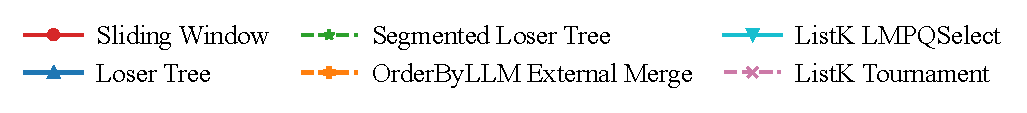
\includegraphics[width=0.88\linewidth]{fig/panels/exp2/exp2_legend.pdf}

  \vspace{-0.3em}

  \subfigure[\Movies (Token)]{
      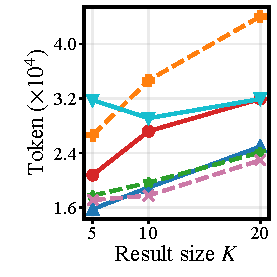
\includegraphics[width=0.33\columnwidth]{fig/panels/exp2/exp2_movies_tokens.pdf}
  }
  \hspace{-2.5ex}
  \subfigure[\Movies (Latency)]{
      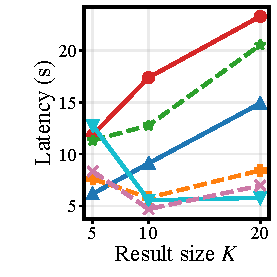
\includegraphics[width=0.33\columnwidth]{fig/panels/exp2/exp2_movies_latency.pdf}
  }
  \hspace{-2.5ex}
  \subfigure[\Movies (nDCG)]{
      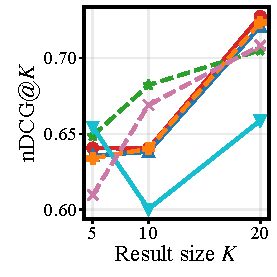
\includegraphics[width=0.33\columnwidth]{fig/panels/exp2/exp2_movies_quality.pdf}
  }

  \subfigure[\DLtwozero (Token)]{
      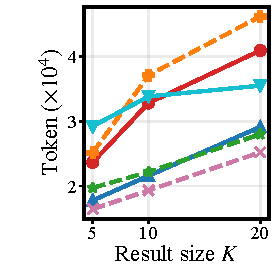
\includegraphics[width=0.33\columnwidth]{fig/panels/exp2/exp2_dl20_tokens.pdf}
  }
  \hspace{-2.5ex}
  \subfigure[\DLtwozero (Latency)]{
      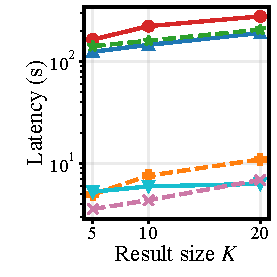
\includegraphics[width=0.33\columnwidth]{fig/panels/exp2/exp2_dl20_latency.pdf}
  }
  \hspace{-2.5ex}
  \subfigure[\DLtwozero (nDCG)]{
      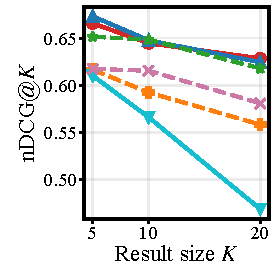
\includegraphics[width=0.33\columnwidth]{fig/panels/exp2/exp2_dl20_quality.pdf}
  }

  \caption{Sensitivity of token cost, latency and nDCG@$K$ in \LIMIT~$K$  by varying $K\in\{5,10,20\}$ ($m{=}10$)}
  \label{fig:exp2-k}
\end{figure}

\Cref{tab:exp1-topk} reports the performance results of \LIMIT~$K$ at $K{=}10$ with the pipeline execution of \cref{sec:topk-exec}. All algorithms retain the default configuration from \cref{sec:exp:full}, isolating the effect of demand-driven execution. \Cref{fig:exp2-k} presents the impact of varying $k$. We evaluate ranking quality (nDCG@10), token cost ($\times 10^3$), and latency (seconds) across six benchmarks: \Movies, \DLtwozero, \DLtwotwo, \COVID, \Touche, and \FiQA. The comparison spans three categories of baselines: pointwise methods (Pointwise, Ext. Pointwise), bubble-based extensions (Ext. Bubble, Ext. Merge), and tournament-style selectors (LMPQSelect, Tournament), against our proposed demand-driven algorithms (\SD, \LT, \SLT).

\noindent \textbf{Quality and efficiency.} Our three algorithms consistently dominate in ranking quality. They claim the top three positions on \DLtwozero, \DLtwotwo, \Touche, and \FiQA; on \Movies, \SD and \LT tie for second. On \COVID they trail only Ext. Bubble and Tournament yet surpass all other baselines. Ext. Bubble and Tournament use acceptance criteria that require repeated comparisons before emitting an item, exposing top-ranked candidates to more competitors and trading higher cost for higher quality. In efficiency, \LT and \SLT match LMPQSelect in token cost while halving that of Ext. Bubble. Demand-driven execution yields dramatic reductions: \LT cuts token consumption by $3$--$5\times$ and latency by $4$--$9\times$ relative to full ranking, as the producer tree propagates only the requested prefix and overlaps adjacent levels without materializing intermediate runs.

\noindent \textbf{The bubble cost-quality trade-off.} Ext. Bubble achieves the highest nDCG on \COVID and strong results elsewhere, but its exhaustive pairwise comparisons incur prohibitive token costs—roughly double those of our \LT variants and an order of magnitude above pointwise methods. This confirms that bubble-based refinement, while accurate, does not scale efficiently.

\noindent \textbf{The pointwise cost-quality trade-off.} Pointwise and Ext. Pointwise minimize token expenditure and latency; Ext. Pointwise even achieves the best average rank in runtime. However, their nDCG scores fall markedly below all competing methods across every dataset. The gap is particularly severe on long-document collections such as \Touche. These results corroborate that pointwise formulations, despite their computational thrift, fail to capture the nuanced relevance signals required for high-quality ranking.

\subsection{Effectiveness of Segmented Loser Tree}
\label{sec:exp:ablation}

% Approved: PR4 cursor/e3-scale-layout-14e8
\begin{figure*}[t]
  \centering
  \includegraphics[width=178mm]{e3-scale.pdf}
  \caption{Synthetic layout for the fixed-$(k,h)$ scale figure, not a measured result.
  The contract names Qwen3.5-9B and one DL20 query; no run produced these heights.
  Input size $n$ is linear at 1k, 5k, and 10k. A logarithmic axis was not specified.
  Each color is one confirmed pair and is the same in the Full and LIMIT~10 panels of that family.
  A solid line with filled circles stands in for a measurement.
  A dashed line stands in for a prediction: the same scaffold plus a constant offset, not a model error.
  Vertical order follows the confirmed list and is not a ranking.
  Open stars are the four LT supplements and are not joined to the five series.
  Full uses $(250,2)$ at 5k and $(500,2)$ at 10k.
  LIMIT~10 uses $(250,1)$ at 5k and $(500,1)$ at 10k.
  Those stars are not per-size optima.
  The vertical unit is a layout unit, not tokens and not a cost.
  Cache off/on is not split, and per-size best $(k,h)$ are omitted.
  Legacy ablation panels in \cref{fig:exp3-ablation} remain until measured results replace them.}
  \label{fig:exp3-scale}
\end{figure*}

\begin{figure}[t]
  \centering

  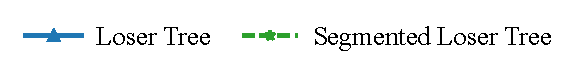
\includegraphics[width=0.65\linewidth]{fig/panels/exp3/exp3_legend.pdf}

  \vspace{-2.0ex}

  \subfigure[\Movies (full rank)]{
      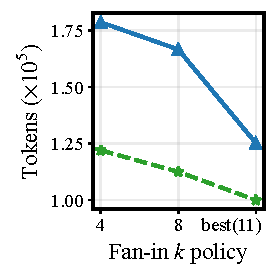
\includegraphics[width=0.33\columnwidth]{fig/panels/exp3/exp3_movies_full_tokens.pdf}
  }
  \hspace{-2.5ex}
  \subfigure[\Movies (full rank)]{
      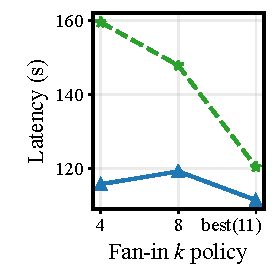
\includegraphics[width=0.33\columnwidth]{fig/panels/exp3/exp3_movies_full_latency.pdf}
  }
  \hspace{-2.5ex}
  \subfigure[\Movies (full rank)]{
      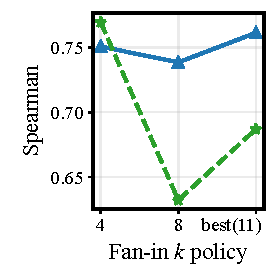
\includegraphics[width=0.33\columnwidth]{fig/panels/exp3/exp3_movies_full_quality.pdf}
  }

  \subfigure[\Movies (\LIMIT~10)]{
      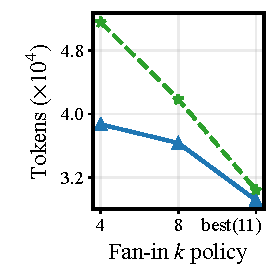
\includegraphics[width=0.33\columnwidth]{fig/panels/exp3/exp3_movies_top10_tokens.pdf}
  }
  \hspace{-2.5ex}
  \subfigure[\Movies (\LIMIT~10)]{
      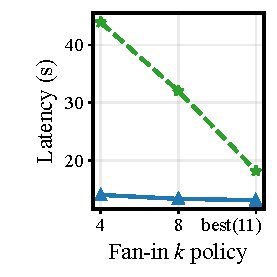
\includegraphics[width=0.33\columnwidth]{fig/panels/exp3/exp3_movies_top10_latency.pdf}
  }
  \hspace{-2.5ex}
  \subfigure[\Movies (\LIMIT~10)]{
      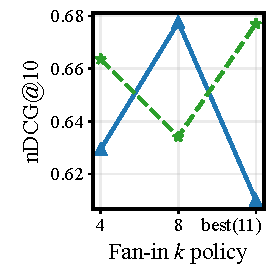
\includegraphics[width=0.33\columnwidth]{fig/panels/exp3/exp3_movies_top10_quality.pdf}
  }

  \subfigure[\DLtwozero (full rank)]{
      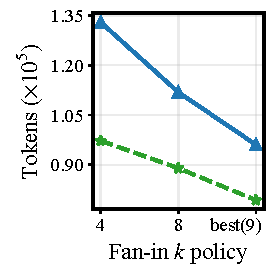
\includegraphics[width=0.33\columnwidth]{fig/panels/exp3/exp3_dl20_full_tokens.pdf}
  }
  \hspace{-2.5ex}
  \subfigure[\DLtwozero (full rank)]{
      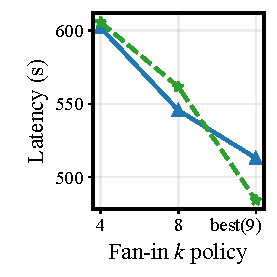
\includegraphics[width=0.33\columnwidth]{fig/panels/exp3/exp3_dl20_full_latency.pdf}
  }
  \hspace{-2.5ex}
  \subfigure[\DLtwozero (full rank)]{
      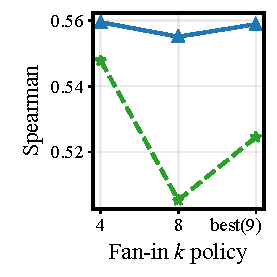
\includegraphics[width=0.33\columnwidth]{fig/panels/exp3/exp3_dl20_full_quality.pdf}
  }

  \subfigure[\DLtwozero (\LIMIT~10)]{
      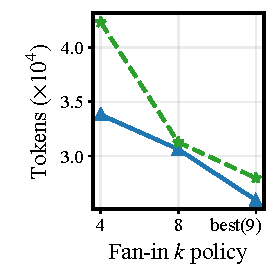
\includegraphics[width=0.33\columnwidth]{fig/panels/exp3/exp3_dl20_top10_tokens.pdf}
  }
  \hspace{-2.5ex}
  \subfigure[\DLtwozero (\LIMIT~10)]{
      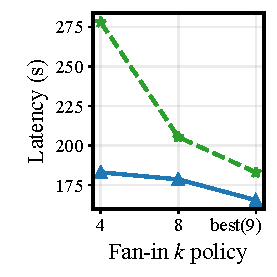
\includegraphics[width=0.33\columnwidth]{fig/panels/exp3/exp3_dl20_top10_latency.pdf}
  }
  \hspace{-2.5ex}
  \subfigure[\DLtwozero (\LIMIT~10)]{
      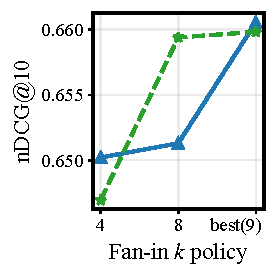
\includegraphics[width=0.33\columnwidth]{fig/panels/exp3/exp3_dl20_top10_quality.pdf}
  }

  \caption{Loser tree vs.\ segmented loser tree under fixed fan-in $k\in\{4,8\}$ and the choice from their cost models}
  \label{fig:exp3-ablation}
\end{figure}
\Cref{fig:exp3-ablation} isolates the effect of segmentation on \Movies and \DLtwozero under both full ranking and \LIMIT~10 settings. \SLT improves listwise throughput by emitting multiple items per listwise call while preserving the global ordering invariant. \SLT improves listwise throughput and consistently reduces token cost by 20\% on average, while latency and ranking quality remain comparable.

\noindent \textbf{Effectiveness of segmentation under \LIMIT~10.}
As \LT emits one item per listwise call, its pipelined merge stops as soon as the requested prefix is complete, avoiding listwise calls on unneeded items. 
Consequently, segmentation is counterproductive under \LIMIT~10: it increases both token cost and latency without a corresponding gain in nDCG.
For both \LT and \SLT on the two datasets, the fan-in $k$ selected by our cost model yields the lowest full ranking token cost. 
We further validate this selection in \cref{sec:exp:cost}.

\subsection{Cost Model Validation}
\label{sec:exp:cost}

% Approved: PR2 cursor/e2-dual-surface-c6cc commit 84a84ad (2x2 main text)
\begin{figure*}[t]
  \centering
  \includegraphics[width=\textwidth]{e2-layout-2x2.pdf}
  \caption{Synthetic layout preview for predicted vs.\ measured token-cost surfaces, not experimental results.
  Blue is measured and orange is predicted.
  Every panel uses the same camera.
  The predicted minimum is drawn at that configuration's measured height; a star on a diamond is both roles at one height.
  Missing corners are left empty.
  The SW column uses the SW legal window ($k\le 20$, $h\le m/k$); the LT column uses the LT window ($k\le 25$, $h$ bounded by max-segment).
  Full and LIMIT10 of one algorithm share that window, including the $z$ ticks.
  The two algorithms are not forced onto one numeric range.
  Panel assignment is not chosen.}
  \label{fig:exp2-surface-2x2}
\end{figure*}

\begin{figure*}[t]
  \centering

  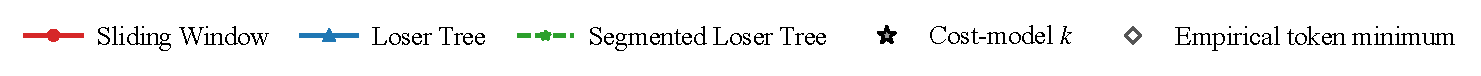
\includegraphics[width=0.75\linewidth]{fig/panels/exp4/exp4_legend.pdf}

  \vspace{-2ex}

  \subfigure[\Movies ($m{=}8$)]{
      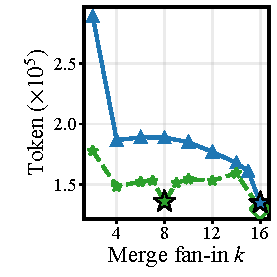
\includegraphics[width=0.33\columnwidth]{fig/panels/exp4/exp4_lt_movies_m8_tokens.pdf}
  }
  \hspace{-2.5ex}
  \subfigure[\DLtwozero ($n ={200}, m{=}10$)]{
      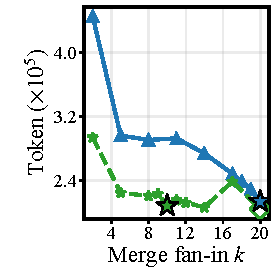
\includegraphics[width=0.33\columnwidth]{fig/panels/exp4/exp4_lt_dl20t200_m10_tokens.pdf}
  }
  \hspace{-2.5ex}
  \subfigure[\DLtwozero ($n{=}500, m{=}12$)]{
      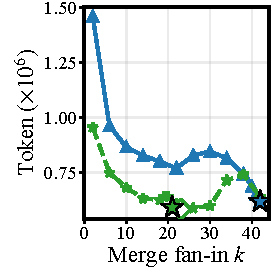
\includegraphics[width=0.33\columnwidth]{fig/panels/exp4/exp4_lt_dl20t500_m12_tokens.pdf}
  }
  \subfigure[\Movies ($m{=}8$)]{
      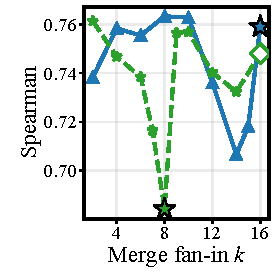
\includegraphics[width=0.33\columnwidth]{fig/panels/exp4/exp4_lt_movies_m8_quality.pdf}
  }
  \hspace{-2.5ex}
  \subfigure[\DLtwozero ($n{=}200, m{=}10$)]{
      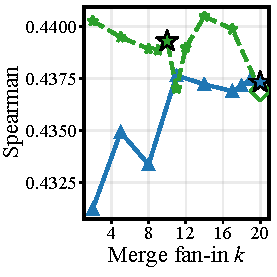
\includegraphics[width=0.33\columnwidth]{fig/panels/exp4/exp4_lt_dl20t200_m10_quality.pdf}
  }
  \hspace{-2.5ex}
  \subfigure[\DLtwozero ($n{=}500,m{=}12$)]{
      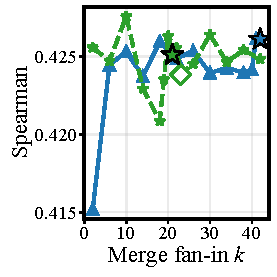
\includegraphics[width=0.33\columnwidth]{fig/panels/exp4/exp4_lt_dl20t500_m12_quality.pdf}
  }

  \subfigure[\Movies ($m{=}12$)]{
      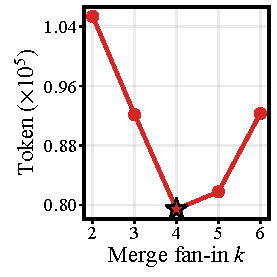
\includegraphics[width=0.33\columnwidth]{fig/panels/exp4/exp4_sw_movies_m12_tokens.pdf}
  }
  \hspace{-2.5ex}
  \subfigure[\DLtwozero ($n{=}500,m{=}20$)]{
      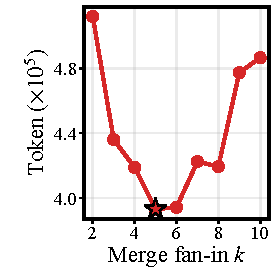
\includegraphics[width=0.33\columnwidth]{fig/panels/exp4/exp4_sw_dl20t500_m20_tokens.pdf}
  }
  \hspace{-2.5ex}
  \subfigure[\DLtwozero ($n{=}500, m{=}30$)]{
      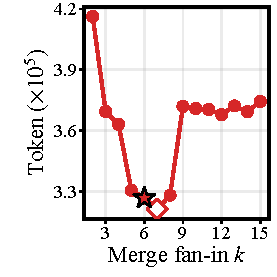
\includegraphics[width=0.33\columnwidth]{fig/panels/exp4/exp4_sw_dl20t500_m30_tokens.pdf}
  }
  \subfigure[\Movies ($m{=}12$)]{
      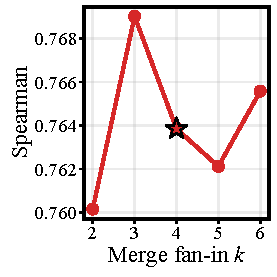
\includegraphics[width=0.33\columnwidth]{fig/panels/exp4/exp4_sw_movies_m12_quality.pdf}
  }
  \hspace{-2.5ex}
  \subfigure[\DLtwozero ($n{=}500,m{=}20$)]{
      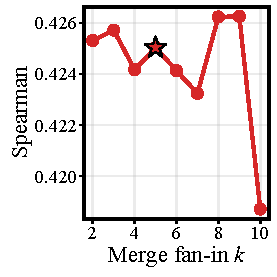
\includegraphics[width=0.33\columnwidth]{fig/panels/exp4/exp4_sw_dl20t500_m20_quality.pdf}
  }
  \hspace{-2.5ex}
  \subfigure[\DLtwozero($n{=}500, m{=}30$)]{
      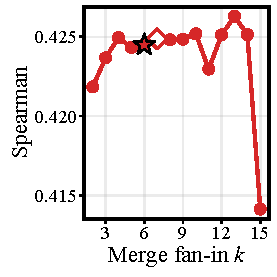
\includegraphics[width=0.33\columnwidth]{fig/panels/exp4/exp4_sw_dl20t500_m30_quality.pdf}
  }

  \caption{Cost model validation: Stars mark the cost model-selected $k_{\mathrm{sel}}$ and diamonds mark the empirical token minimum $k$.}
  \label{fig:exp4-full}
\end{figure*}

\begin{figure}[t]
  \centering

  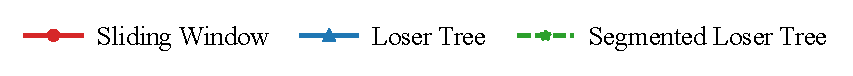
\includegraphics[width=0.88\linewidth]{fig/panels/exp4/exp4_topk_legend.pdf}

  \vspace{-0.4em}

  \subfigure[\Movies]{
      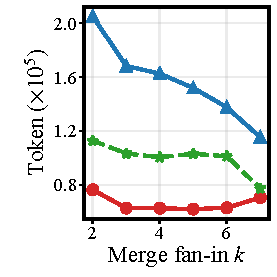
\includegraphics[width=0.25\columnwidth]{fig/panels/exp4/exp4_topk_movies_m20_tokens.pdf}
  }
  \hspace{-2.6ex}
  \subfigure[\Movies ]{
      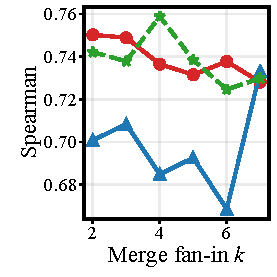
\includegraphics[width=0.25\columnwidth]{fig/panels/exp4/exp4_topk_movies_m20_quality.pdf}
  }
\hspace{-2.6ex}
  \subfigure[\DLtwozero]{
      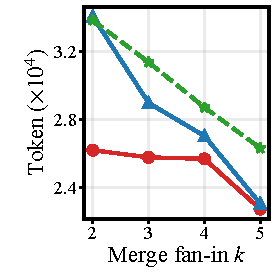
\includegraphics[width=0.25\columnwidth]{fig/panels/exp4/exp4_topk_dl20_m20_tokens.pdf}
  }
  \hspace{-2.6ex}
  \subfigure[\DLtwozero]{
      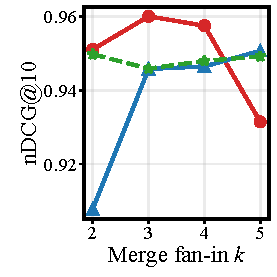
\includegraphics[width=0.25\columnwidth]{fig/panels/exp4/exp4_topk_dl20_m20_quality.pdf}
  }

  \caption{Sensitivity of fan-in $k$ under \LIMIT~10}
  \label{fig:exp4-topk}
\end{figure}

\begin{figure*}[t]
  \centering

  
\includegraphics[width=0.8\linewidth]{fig/panels/exp5/exp5_legend.pdf}

  \vspace{-2ex}

  \subfigure[\Movies (full rank)]{
      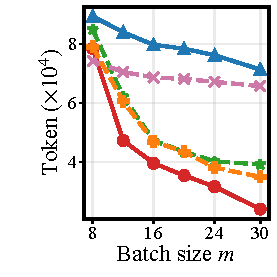
\includegraphics[width=0.33\columnwidth]{fig/panels/exp5/exp5_movies_full_tokens.pdf}
  }
  \hspace{-2.5ex}
  \subfigure[\Movies (full rank)]{
      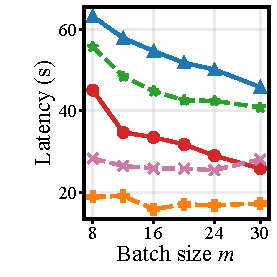
\includegraphics[width=0.33\columnwidth]{fig/panels/exp5/exp5_movies_full_latency.pdf}
  }
  \hspace{-2.5ex}
  \subfigure[\Movies (full rank)]{
      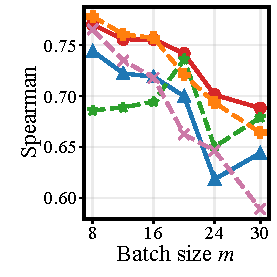
\includegraphics[width=0.33\columnwidth]{fig/panels/exp5/exp5_movies_full_quality.pdf}
  }
  \subfigure[\Movies (\LIMIT~$10$)]{
      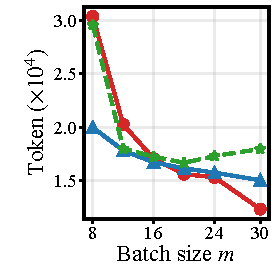
\includegraphics[width=0.33\columnwidth]{fig/panels/exp5/exp5_movies_top10_tokens.pdf}
  }
  \hspace{-2.5ex}
  \subfigure[\Movies (\LIMIT~$10$)]{
      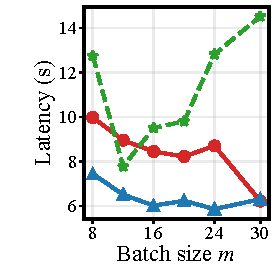
\includegraphics[width=0.33\columnwidth]{fig/panels/exp5/exp5_movies_top10_latency.pdf}
  }
  \hspace{-2.5ex}
  \subfigure[\Movies (\LIMIT~$10$)]{
      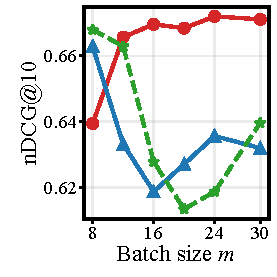
\includegraphics[width=0.33\columnwidth]{fig/panels/exp5/exp5_movies_top10_quality.pdf}
  }

  \subfigure[\DLtwozero (full rank)]{
      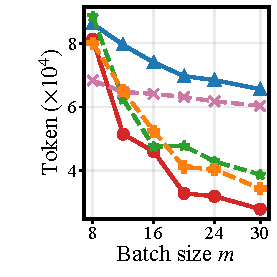
\includegraphics[width=0.33\columnwidth]{fig/panels/exp5/exp5_dl20_full_tokens.pdf}
  }
  \hspace{-2.5ex}
  \subfigure[\DLtwozero (full rank)]{
      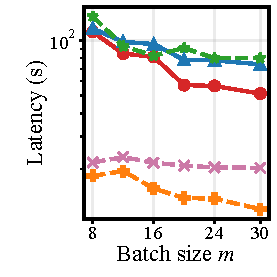
\includegraphics[width=0.33\columnwidth]{fig/panels/exp5/exp5_dl20_full_latency.pdf}
  }
  \hspace{-2.5ex}
  \subfigure[\DLtwozero (full rank)]{
      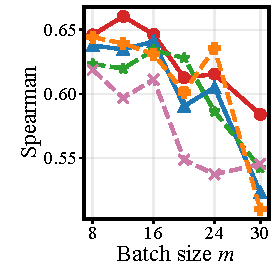
\includegraphics[width=0.33\columnwidth]{fig/panels/exp5/exp5_dl20_full_quality.pdf}
  }
  \subfigure[\DLtwozero (\LIMIT~$10$)]{
      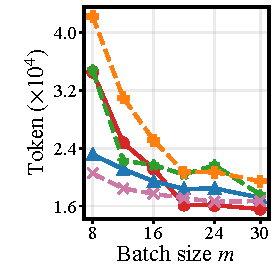
\includegraphics[width=0.33\columnwidth]{fig/panels/exp5/exp5_dl20_top10_tokens.pdf}
  }
  \hspace{-2.5ex}
  \subfigure[\DLtwozero (\LIMIT~$10$)]{
      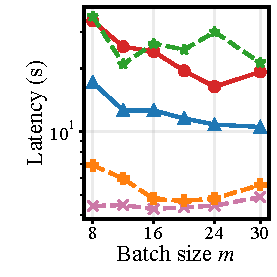
\includegraphics[width=0.33\columnwidth]{fig/panels/exp5/exp5_dl20_top10_latency.pdf}
  }
  \hspace{-2.5ex}
  \subfigure[\DLtwozero (\LIMIT~$10$)]{
      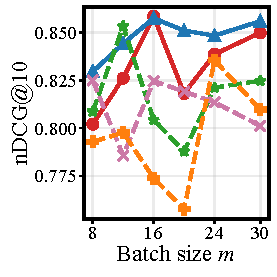
\includegraphics[width=0.33\columnwidth]{fig/panels/exp5/exp5_dl20_top10_quality.pdf}
  }

  \caption{Impact of listwise batch size $m$ on cost, latency and quality}
  \label{fig:exp5-m}
\end{figure*}


We evaluate the impact of fan-in $k$ on token cost and ranking quality for our three algorithms across three datasets.
For each algorithm, we sweep $k$ at two fixed batch sizes $m$, with both full ranking and \textsc{Limit}~$K{=}10$. 
For full ranking, we mark the cost-model-selected $k_a^\star$ on each sweep curve. 
Results show $k_a^\star$ precisely matches with the empirical token optimum $k^*$ or lies near it. $k_a^\star=k^*$ occurs in five of all six settings, with the remaining mismatched setting's token regret at most $1.99\%$. 
This confirms our cost model effectively selects the cost-optimal $k$.

\noindent \textbf{Token cost vs.\ fan-in.}
\LT exhibits monotonically decreasing token cost as $k$ increases, reaching minimum at $k=r$. In contrast, \SD and \SLT show U-shaped curves: cost first decreases then increases with $k$, yielding an interior minimum. For \SD, this reflects the trade-off between fewer merge rounds (larger $k$) and higher per-round prompt complexity. \SLT balances larger segments against segmented structure overhead. The per-pass cost of \LT is nearly independent of $k$, which is deduced in~\cref{subsec:cost-loser-tree}, so minimizing the number of passes is optimal, with $k{=}r$ completing the merge in one pass. On \Movies at $m{=}8$, the selected fan-in saves $27.8\%$ for \LT and $8.5\%$ for \SLT relative to $k{=}4$; \SD saves $21.5\%$--$24.6\%$ relative to $k{=}2$. Larger deviations at $m{=}8$ occur in narrow feasible ranges.

\noindent \textbf{Ranking quality vs.\ fan-in.}
Fan-in affects quality far less than cost. At selected $k_a^\star$, quality remains close to the best measured value in all settings except \LT on \Movies at $m{=}8$. Quality curves show no consistent trend with $k$, indicating cost-driven selection introduces no systematic quality loss. Thus optimizing $k$ for token cost preserves ranking effectiveness.


\subsection{LIMIT $n$ sensitivity (layout integration)}
\label{sec:exp:limit-sweep}

% Parent-approved LIMIT-n sweep layouts (synthetic); does not replace fig:exp5-m.
% E5: Off + On-cold on one float page (proportional scale; aspect preserved).
\begin{figure*}[t]
  \centering
  \subfigure[Cache Off (\(\beta{=}0\), \(U\) cost scale).]{%
    \includegraphics[width=\linewidth,height=0.38\textheight,keepaspectratio]{e5-limit-sweep-off.pdf}%
    \label{fig:exp5-k-sweep-off}}%
  \subfigure[Cache On-cold (measured \(U{-}Q\) scale).]{%
    \includegraphics[width=\linewidth,height=0.38\textheight,keepaspectratio]{e5-limit-sweep-on.pdf}%
    \label{fig:exp5-k-sweep-on}}%
  \caption{Synthetic layout---not experimental results. LIMIT~$n$ contract: equal category spacing (not linear in $n$); Full isolated; LIMIT~500 is last connected point.}
\end{figure*}

\subsection{Impact of Listwise Batch Size}
\label{sec:exp:m}



\Cref{fig:exp5-m} studies the impact of the listwise batch size $m$ on token cost, latency, and ranking quality for both full-ranking and \LIMIT~10 workloads on \Movies and \DLtwozero.
Five merge algorithms are evaluated under the same batch sizes setting.
Overall, increasing $m$ exposes a clear trade-off between token cost and quality.
Larger batch size reduces the number of LLM invocations and token consumption, but they also make each invocation more difficult for the LLM.
As a result, full-ranking quality gradually deteriorates as $m$ increases, while latency exhibits a non-monotonic trend because the reduction in invocation count competes with the increasing cost of each individual LLM call.


\noindent \textbf{Impact of batch size $m$ on token cost and quality.}
Increasing $m$ consistently reduces token cost across all algorithms.
The reason is straightforward: a larger listwise batch ranks more items in each LLM invocation, thereby reducing both the number of initial runs ($r=\lceil n/m\rceil$) and the subsequent merge operations.
This reduction in token cost comes at the expense of ranking quality.
As $m$ grows, each LLM call must jointly order more candidates within a single context, making the ranking task increasingly challenging and introducing more ordering errors.
These errors accumulate throughout the merge process and are reflected by the full-ranking Spearman metric.
In contrast, \LIMIT~10 remains relatively stable because only the highest-ranked items are evaluated, making errors in the tail of the ranking largely invisible.


\noindent \textbf{Impact of batch size $m$ on latency.}
The effect of $m$ on latency is more nuanced.
Increasing $m$ reduces the number of LLM invocations almost linearly, which tends to lower the overall execution time.
However, each invocation becomes substantially more expensive because a larger batch produces a longer prompt and requires the LLM to reason over more candidates simultaneously.
The computational cost of Transformer attention increases superlinearly with the input length during prompt processing, while longer prompts also increase the amount of decoding tokens.
Consequently, the increased latency of each individual call can offset, or even outweigh, the reduction in invocation count.

